\documentclass{article}
\usepackage{../tex/mysty}
\usepackage[final]{pdfpages}
\begin{document}


\maketitlepage{U.S. Food and Drug Administration: Regulatory
  Report}{Sanjay Challa}

\setcounter{tocdepth}{3}
\tableofcontents
\newpage

\section*{Executive summary}
\label{sec:exec-summary}

\section{Regulation Overview}
\label{sec:test-administration}

\section{Device Classification}
\label{sec:protocols}
B. Device Classification Wt =20% Points ____
a. Panels ______
b. 7-digit classification ______
c. 3-alpha code ______
d. Documentation on how search was conducted ______
e. If not regulated, state compelling argument ______
f. What other regulations may apply? ______
A search in the PRODUCT CODE CLASSIFICATION DATABASE using the keywords: "tomography" and "ophthalmic", is done. There are few entrys that partially describes our device. Optical coherence tomography, product code OBO, regulation number 886.1570, describes an ophthalmoscope as an "Diagnostic device to aid in the detection and management of various ocular diseases" capable of "viewing, imaging, measurement, and analysis of ocular structures."  Computed tomography x-ray system, product code JAK, regulation number 892.1750, describes a diagnostic x-ray system of similar technicality to our device. Either of the definition does not fully describe our device and the major difference lies in that our device is not intended for any diagnotics purposes.
Even thought there are existing classified devices that partially describe our device, our device is most likely not regulated by the FDA as medical device. According to the FD&C Act, a "device" is "an instrument, apparatus, implement, machine, contrivance, implant, in vitro reagent, or other similar or related article, including any component, part, or accessory, which is:(1) recognized in the official National Formulary, or the United States Pharmacopeia, or any supplement to them,
(2) intended for use in the diagnosis of disease or other conditions, or in the cure, mitigation, treatment, or prevention of disease, in man or other animals, or
(3) intended to affect the structure or any function of the body of man or other animals, and which does not achieve its primary intended purposes through chemical action within or on the body of man or other animals and which is not dependent upon being metabolized for the achievement of its primary intended purposes." (Cite FD&C Act 21USC321)
Our device clearly does not fit the second and third definition. It is not inteneded for any use in or affect the structure or functionality of any part of a living organism. An item by item search in Title 21 of the Code of Federal Regulations (CFR), Parts 886,ophthalmic panel and 892 radiological panel, confirms that there our device is not substantially equivalent to any of the existing devices. Our device has similar technological characteristic to but does not have the same intended use as the two entried mentioned above.
However, considering the presence of electronic and visible radiation emitting component in our device, regulations in the FD&C Act sections 531-542 Electronic Product Radiation Control provisions is still applicable to our device.
\addcontentsline{toc}{section}{510(k) Premarket Notification}
% Cover sheets
\addcontentsline{toc}{subsection}{CDRH Premarket Review Submission Cover Sheet}

\begin{figure}[H]
  \centering
  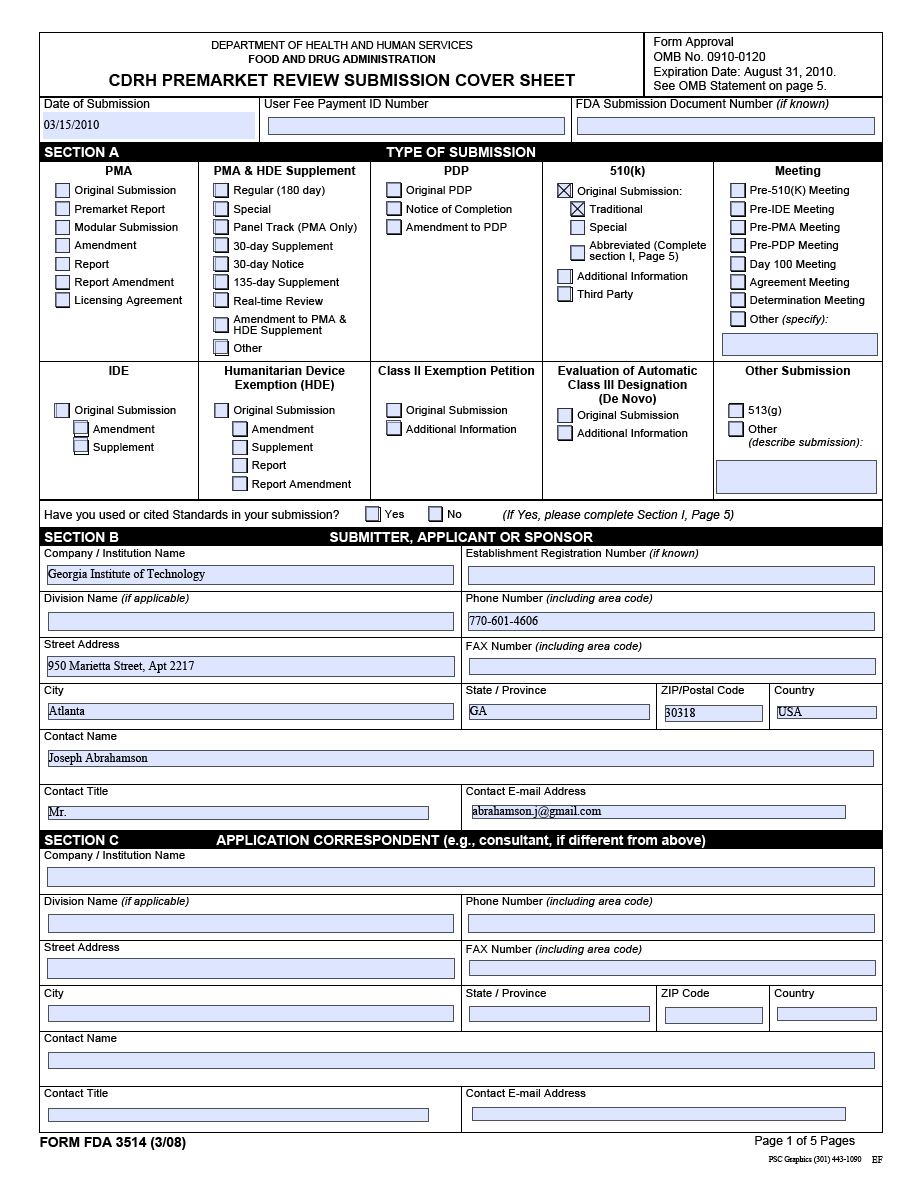
\includegraphics[width=1.2\linewidth]{pages/cdrh-pics/1}
  \label{fig:summary}
\end{figure}

\begin{figure}[H]
  \centering
  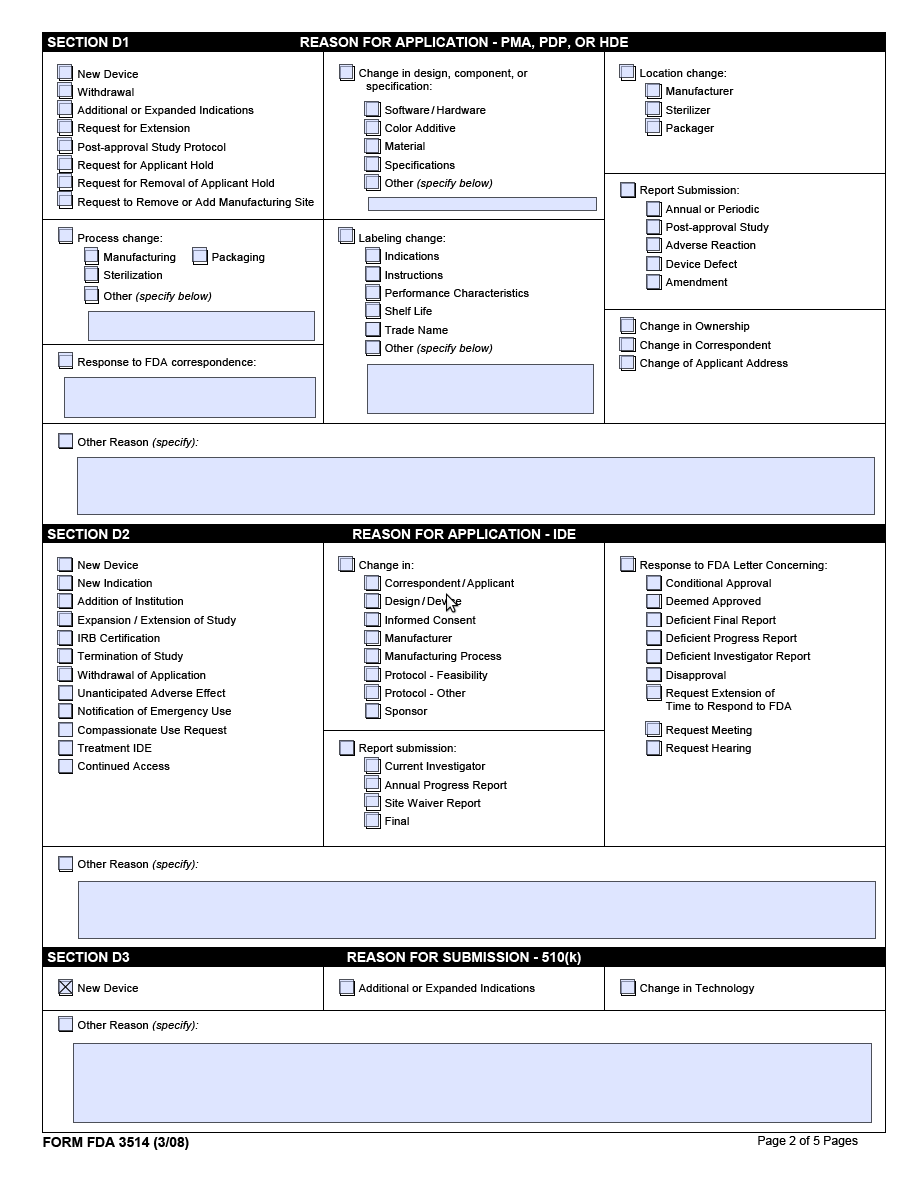
\includegraphics[width=1.2\linewidth]{pages/cdrh-pics/2}
  \label{fig:summary}
\end{figure}

\begin{figure}[H]
  \centering
  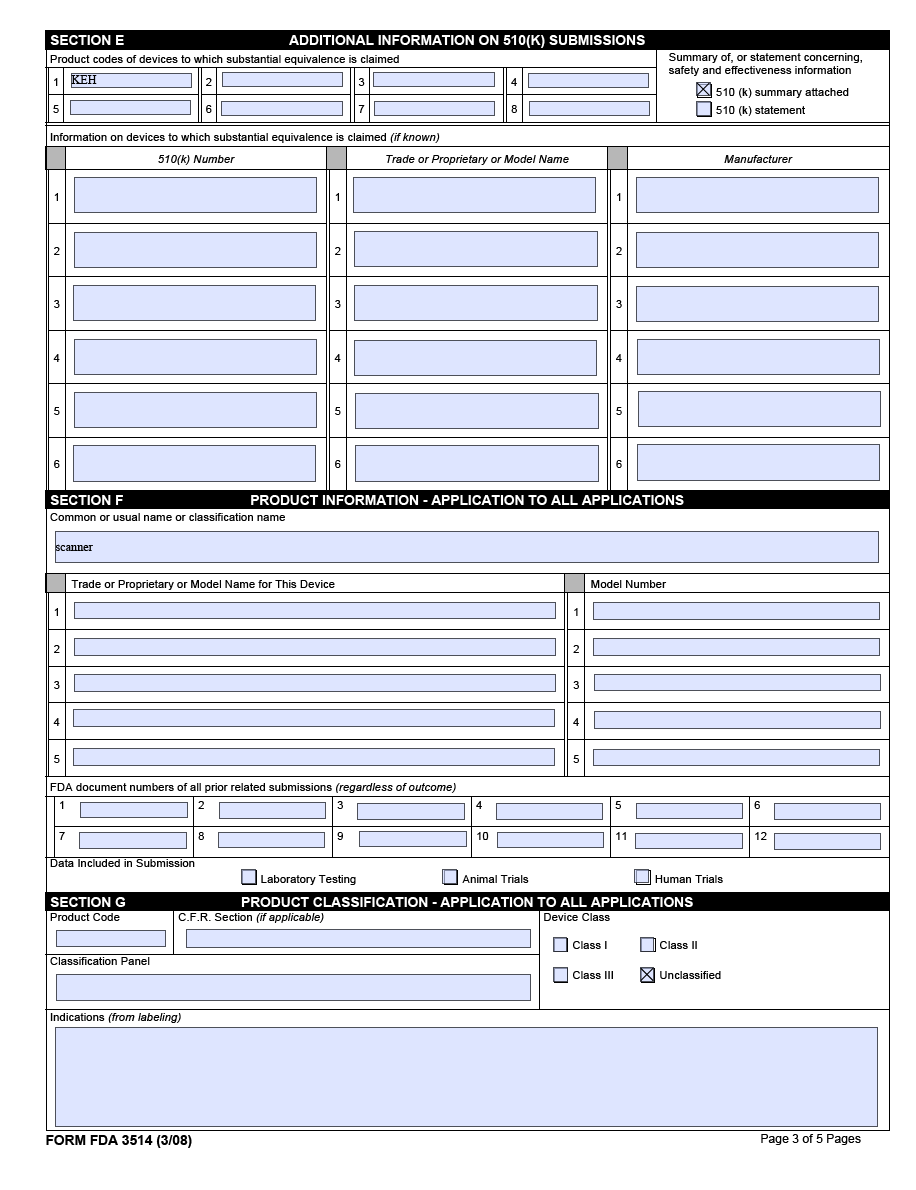
\includegraphics[width=1.2\linewidth]{pages/cdrh-pics/3}
  \label{fig:summary}
\end{figure}

\begin{figure}[H]
  \centering
  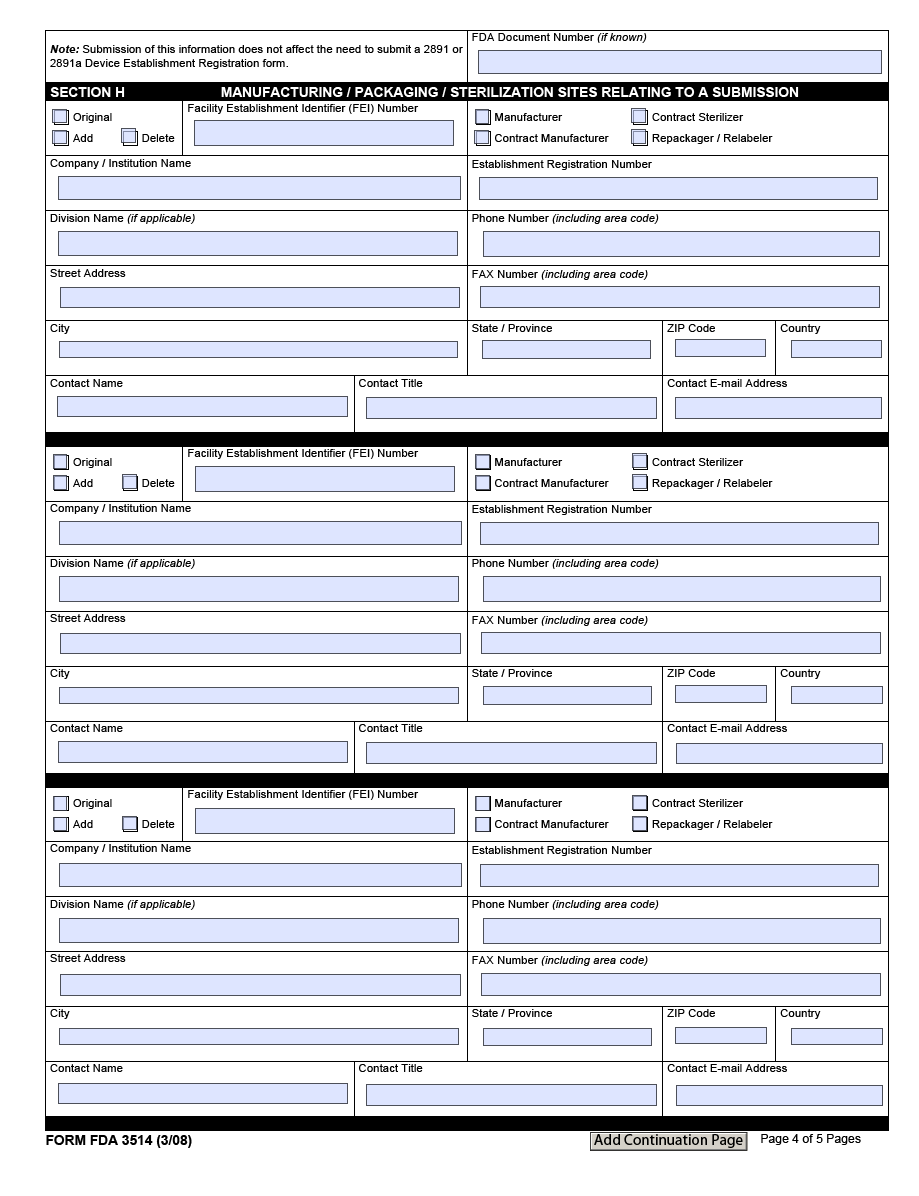
\includegraphics[width=1.2\linewidth]{pages/cdrh-pics/4}
  \label{fig:summary}
\end{figure}

\begin{figure}[H]
  \centering
  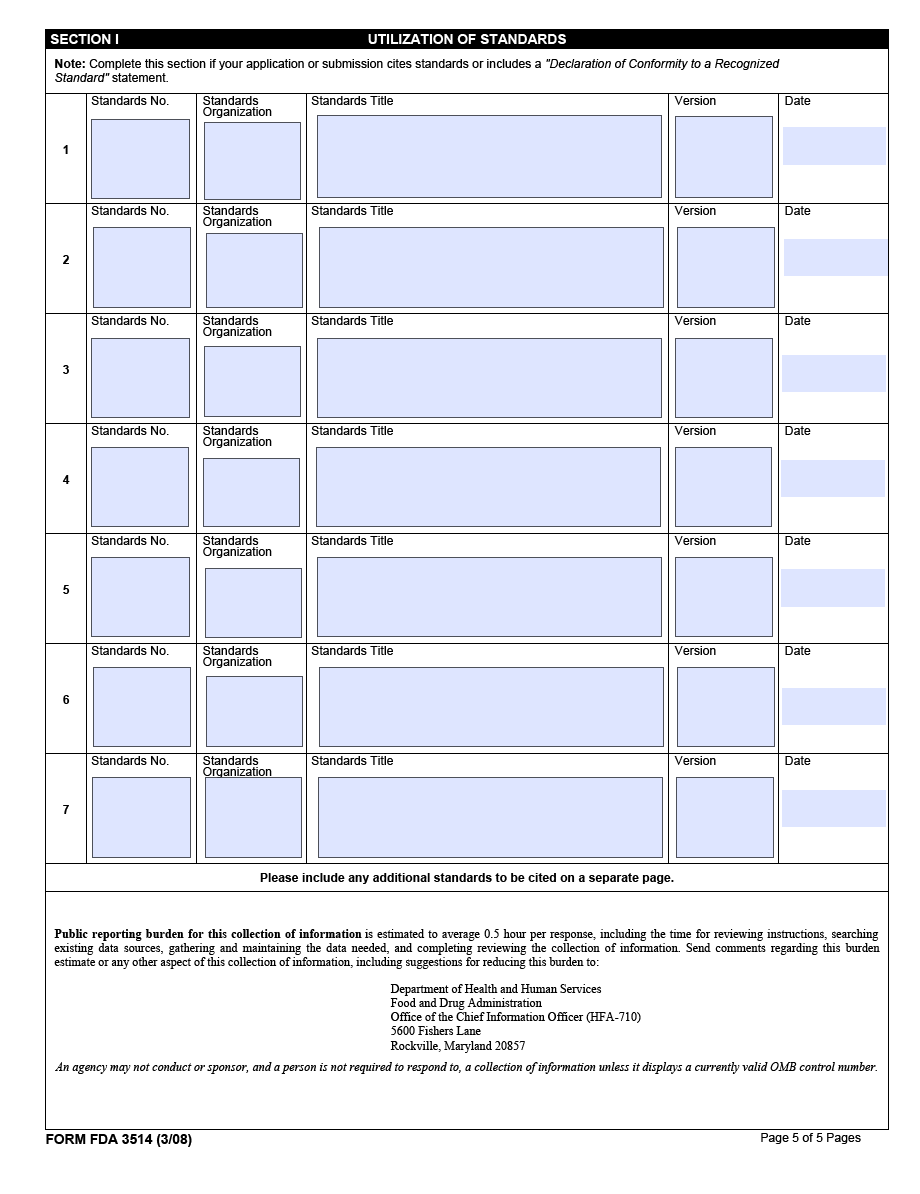
\includegraphics[width=1.2\linewidth]{pages/cdrh-pics/5}
  \label{fig:summary}
\end{figure}

%%% Local Variables: 
%%% mode: latex
%%% TeX-master: "../reg"
%%% End: 

\newpage
\addcontentsline{toc}{subsection}{510(k) Cover Letter}
\singlespacing

\begin{flushright}
  \huge{510(k) Submission --- Traditional}\\[.5in]
  
  \begin{minipage}{0.8\textwidth}
    \begin{flushright}
      \large \textbf{Scanner: eyeScan Mezzo} \\
      \textit{\today}
    \end{flushright}
  \end{minipage}
\end{flushright}

\begin{flushleft}
  Joseph Abrahamson\\
  $<$\textit{abrahamson.j@gatech.edu}$>$ \\
  Phone: 770 601 4606 \\[1em]
  
  \textit{Will register establishment following FDA clearance.}
\end{flushleft}
\vspace{4em}

\onehalfspacing

We seek FDA clearance to market our device, \textbf{eyeScan Mezzo}, a
Class II medical device used for medical scanning of three-dimensional
exterior eye shape. To our knowledge FDA has not classified this
device and, thus, no product code has been assigned or requested for
this device in the Classification Database. Substantially equivalent
devices belong to the General \& Plastic Surgery, Radiology, and
Pathology panels. This finished component is a novel device not
previously marketed with FDA clearance in the USA. We require 510(k)
clearance due to substantial equivalence with existent optical
coherence tomography devices (regulation no. \textbf{886.1570},
product code \textbf{OBO}), x-ray computed tomography devices
(regulation no. \textbf{892.1750}, product code \textbf{JAK}), and
microscopes, micrometers, and accessories (regulation
no. \textbf{864.3600}, product code \textbf{KEH}). Manufacturing
registration is currently unspecified. 

With regards to performance standards, this device contains electrical
components, and is subject to testing under IEC 60601-1-2 Part
I. Furthermore, the device contains a laser component, which under 21
CFR 1000 dictates that the device falls under RCHSA controls. RCHSA
controls indicate that the manufacture of the laser component of this
device is subject to standards 1002.10, 1002.13, and 1002.30, which
specifiy necessary reporting on the manufacturing of the laser
component. Lastly, while the device does contain a laser, it is exempt
from 21 CFR 1040.

%%% Local Variables: 
%%% mode: latex
%%% TeX-master: "../reg"
%%% End:



% Real sections
\setcounter{subsection}{0}
\newpage
\addcontentsline{toc}{subsection}{Indications for Use Statement}

\begin{center}
  \huge{Indications for Use Statement}\\[.5in]
\end{center}


\onehalfspacing

510(k) Number (if known): N/A \\
Device Name: eyeScan Mezzo \\
Indications for Use: 

%%% Local Variables: 
%%% mode: latex
%%% TeX-master: "../reg"
%%% End: 


\subsection{510(k) Summary}
\subsection{Truthful and Accuracy Statement}
\subsection{Class III Summary and Certification}
\subsection{Financial Certification or Disclosure Statement}
\subsection{Declarations of Conformity and Summary Reports}
\subsection{Executive Summary}
\subsection{Device Description}
\subsection{Substantial Equivalence Discussion}
\subsection{Proposed Labeling}
\subsection{Sterilization and Shelf Life}
\subsection{Biocompatibility}
\subsection{Software}
\subsection{Electromagnetic Compatibility and Electrical Safety}
%\subsection{Performance Testing --- Lab, Animal, Clinical}
% Not required

\section{Discussion}
\label{sec:discussion}

\section{Conclusion}
\label{sec:conclusion}


\newpage
\addcontentsline{toc}{section}{References}
\bibliographystyle{unsrt}
\bibliography{../tex/bibl}

\end{document}
%%% Local Variables: 
%%% mode: latex
%%% TeX-master: t
%%% End: 
